\documentclass[crop,tikz,border=1px]{standalone}

\usetikzlibrary{arrows,positioning,scopes,automata,calc}

\begin{document}
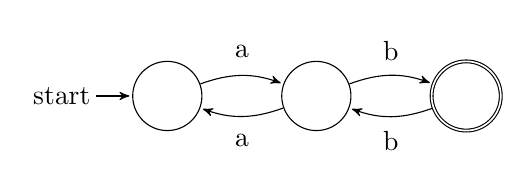
\begin{tikzpicture}[->,>=stealth',shorten >=1pt,auto,
  inner sep=2pt,minimum size=.6cm,
  mystate/.style={state,text centered}]

  \node[initial,mystate] (q0) {};
  \node[mystate] (q1) [right=of q0] {};
  \node[accepting,mystate] (q2) [right=of q1] {};

  {[every edge/.append style={bend left=20}]
    \foreach \a/\i/\b in {q0/a/q1, q1/b/q2} {
      \path (\a) edge node [above] {\i} (\b)
            (\b) edge node [below] {\i} (\a);
    }
  }

\end{tikzpicture}
\end{document}
